%-----------------------------------------
\begin{frame}
\frametitle{Tangible illustration of problem}
\centering
Useful in combination?\\
Need to wait for downscale for improvement?
\begin{minipage}{0.45\textwidth}
    \begin{figure}      
    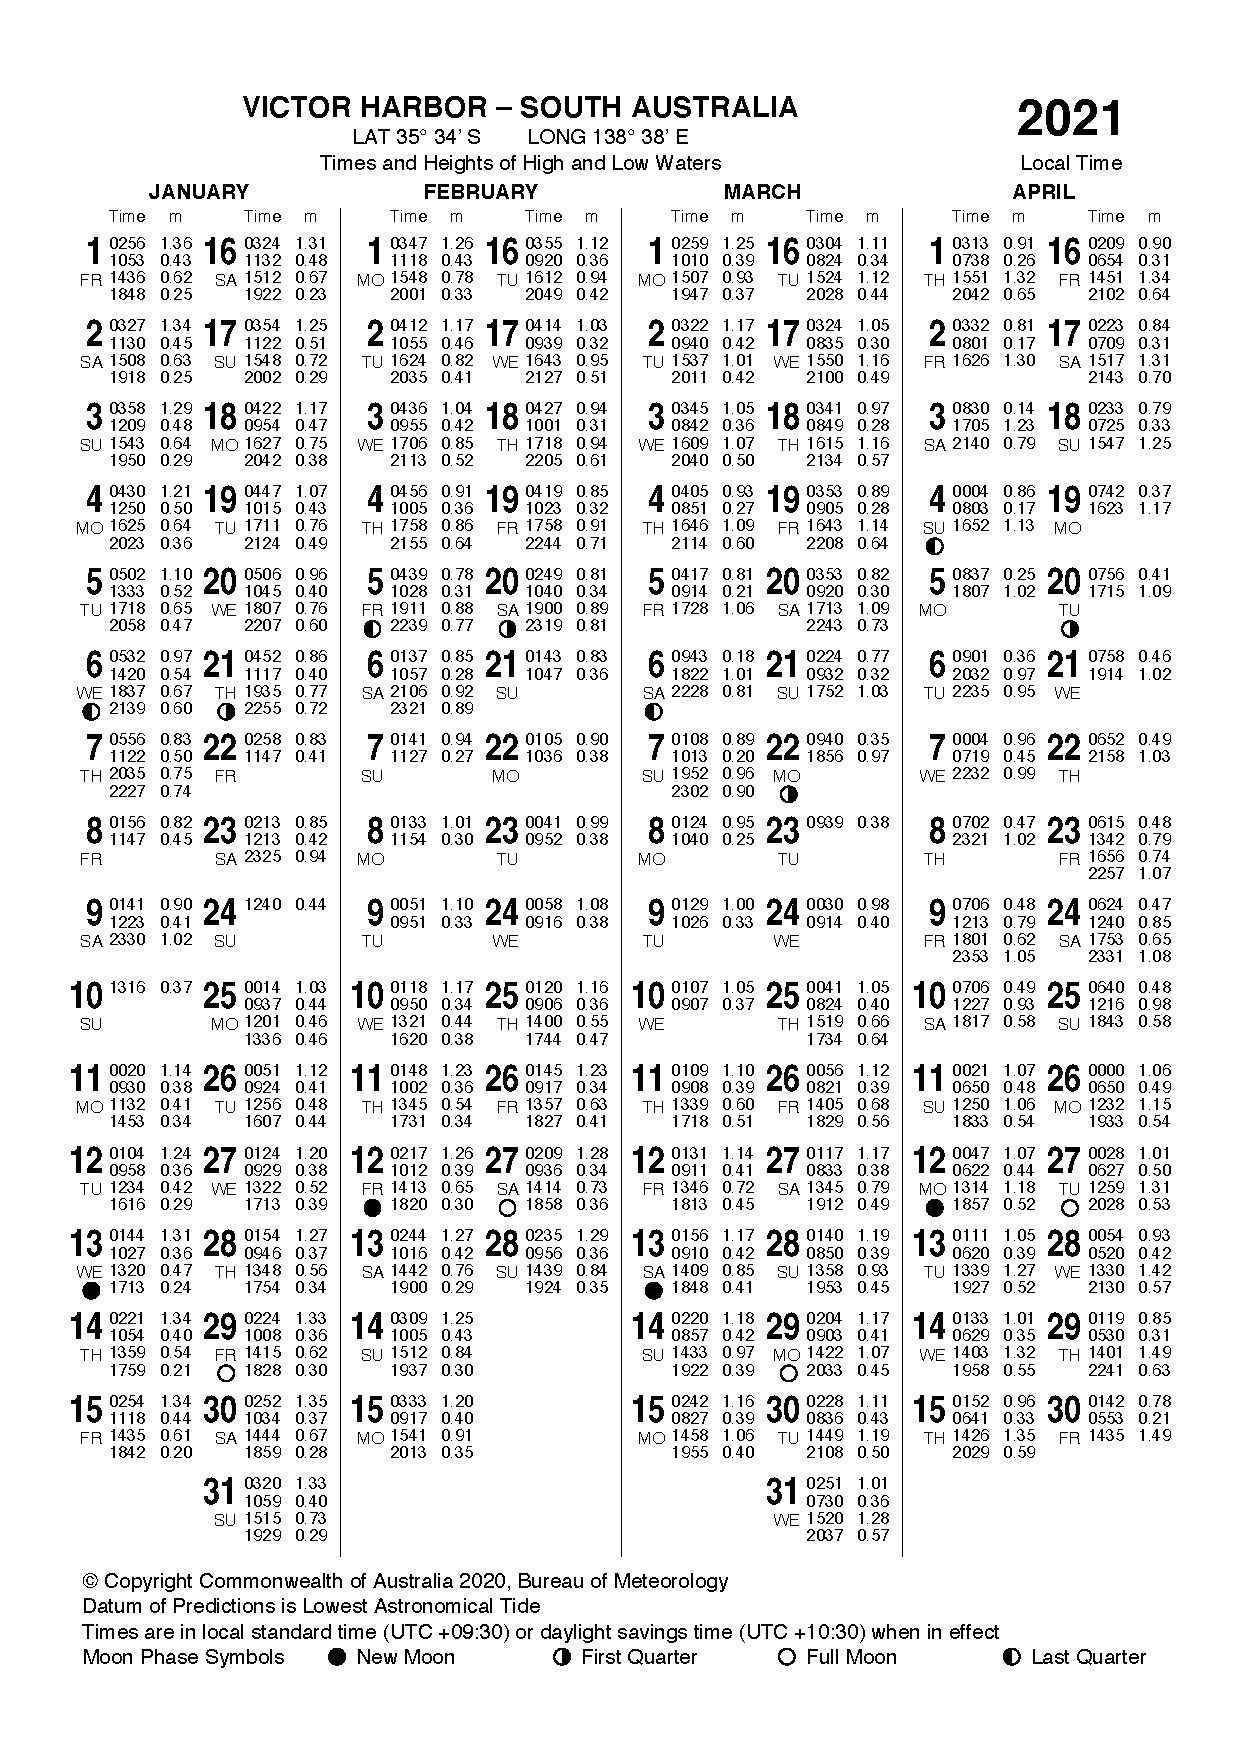
\includegraphics[trim={0 8cm 0 0},clip,height=\textheight]{figures/images/IDO59001_2021_SA_TP006.pdf}
    \end{figure}
\end{minipage}
\hfill
\begin{minipage}{0.45\textwidth}
    \begin{figure}      
     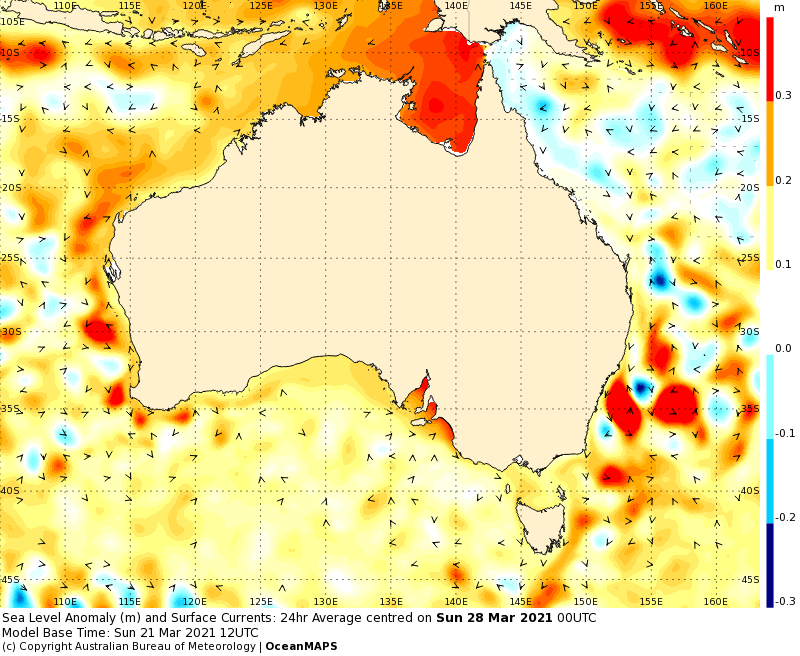
\includegraphics[width=\textwidth]{figures/images/IDYOC300.Aus.SLACur.168.png}
    \end{figure} 
\end{minipage}
\end{frame}
%-----------------------------------------
\begin{frame}
\frametitle{Tangible illustration of problem}
Longer forecast window versus detail.\\
Non-extreme management.\\
\begin{minipage}{0.4\textwidth}
    \begin{figure}      
    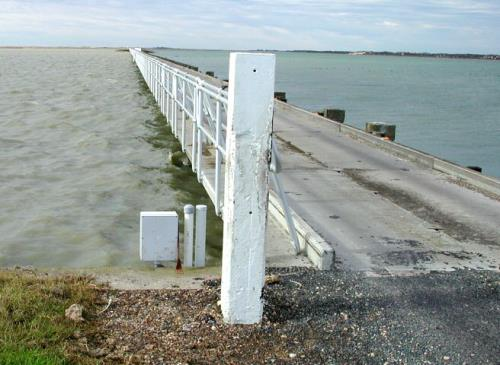
\includegraphics[height=0.4\textheight]{figures/images/goolwa_ewe_island-environment_sa_gov_au.jpg}
    \end{figure}
\end{minipage}
\hfill
\begin{minipage}{0.4\textwidth}
    \centering
     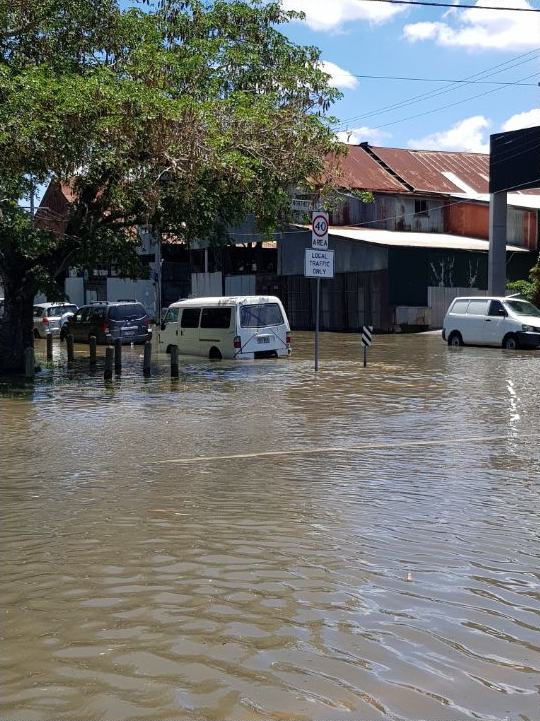
\includegraphics[width=0.8\textwidth]{figures/images/sunnyFlood_ClarkJan2018Brisbane.png} 
\end{minipage}

\end{frame}
%-----------------------------------------
\begin{frame}
\frametitle{Tangible illustration of problem}

\begin{minipage}{0.6\textwidth} 
\centering
      sea level and positioning\\
      
      
      tidal planes for elevation\\
      
      
      standard tides as reference\\
      
      
      boundary conditions, down-scaling
\end{minipage}
\begin{minipage}{0.3\textwidth}
    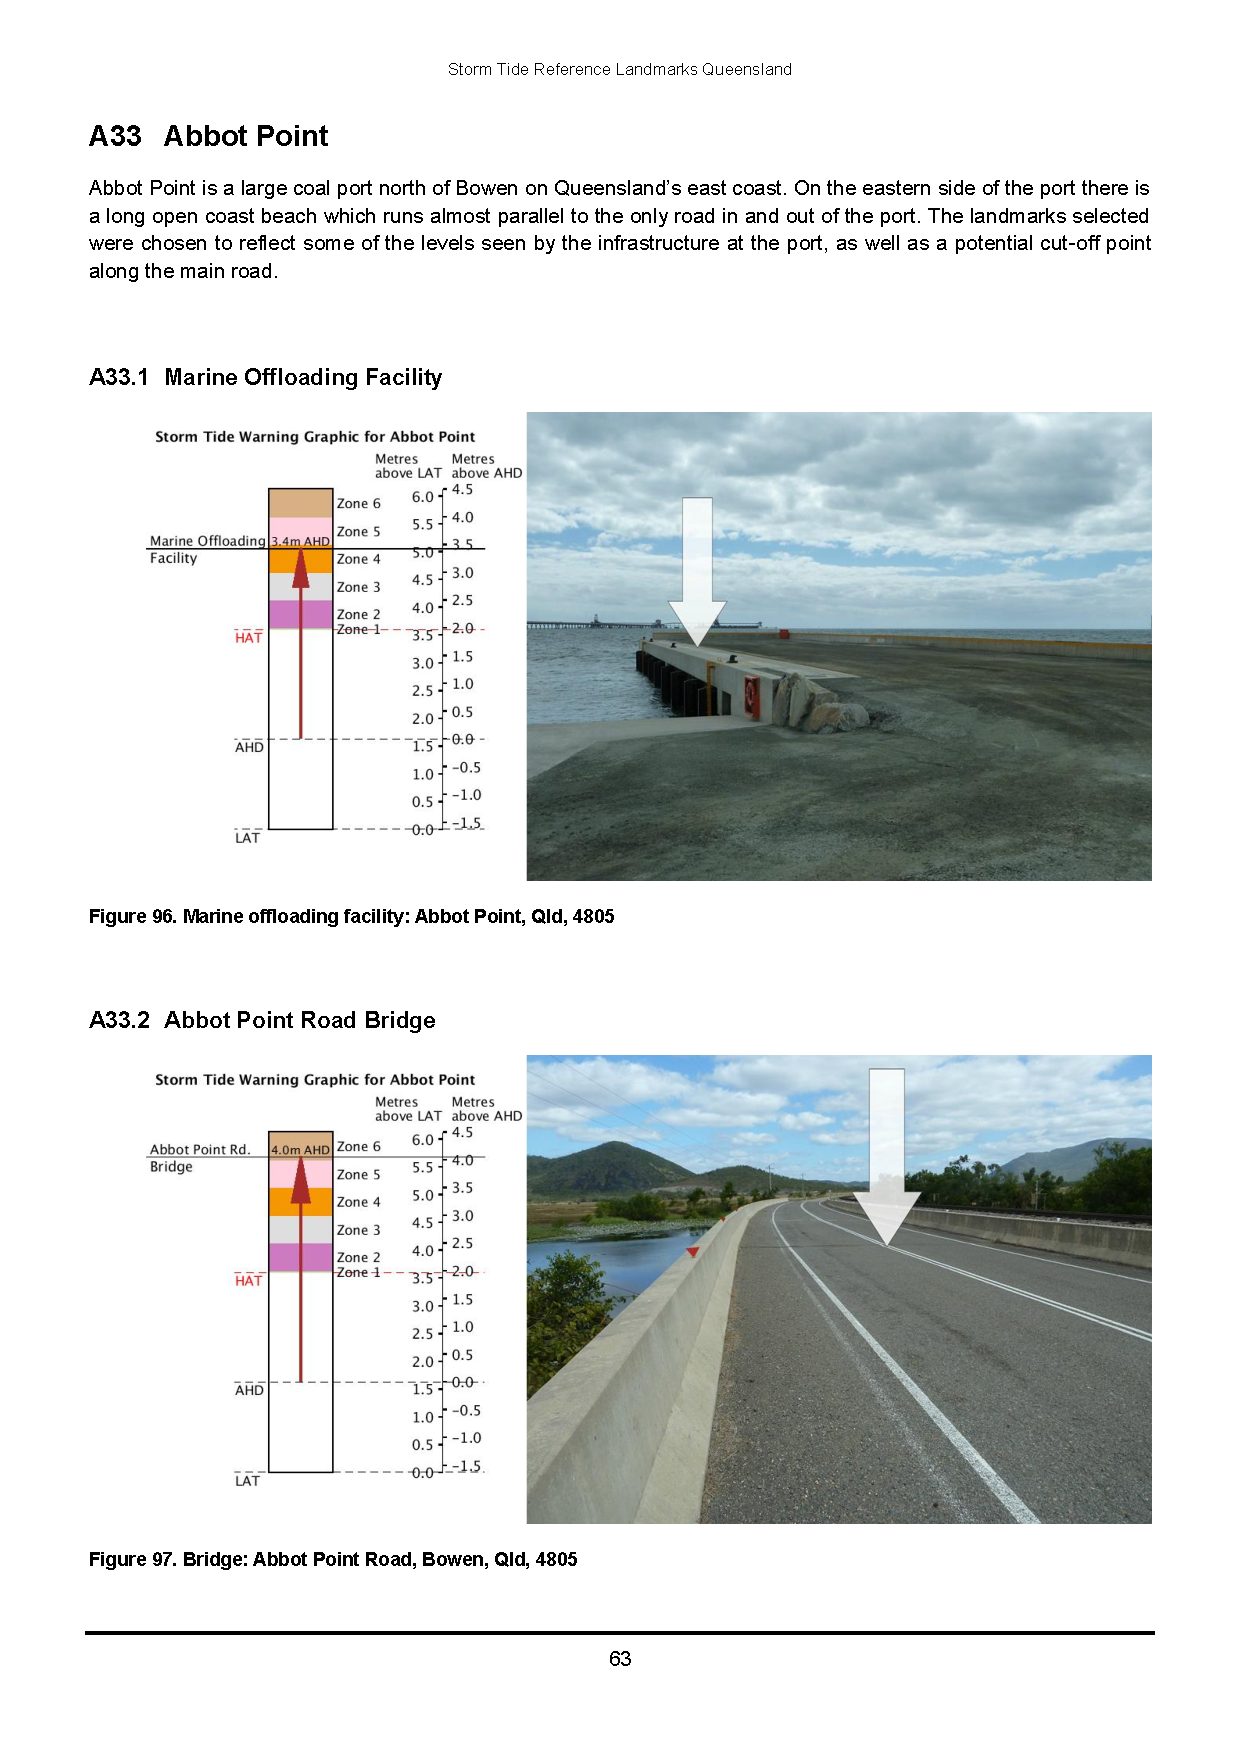
\includegraphics[trim={2cm 0 5cm 5cm},clip,height=0.9\textheight]{figures/images/qldLandmarkEg.pdf}
\end{minipage}

\end{frame}

